\begin{frame}
\frametitle{Participate!}
During the lectures...
\begin{itemize}
\item Don't hesitate to ask questions. Other people in the audience may have
similar questions too.
\item This helps the trainer to detect any explanation that wasn't clear or
detailed enough.
\item Don't hesitate to share your experience, for example to compare Linux
/ Android with other operating systems used in your company.
\item Your point of view is most valuable, because it can be similar to your
colleagues' and different from the trainer's.
\item Your participation can make our session more interactive and make the
topics easier to learn.
\end{itemize}
\end{frame}

\begin{frame}
\frametitle{Practical lab guidelines}
During practical labs...
\begin{itemize}
\item We cannot support more than 8 workstations at once (each with its board
and equipment). Having more would make the whole class progress slower,
compromising the coverage of the whole training agenda (exception for public
sessions: up to 10 people).
\item So, if you are more than 8 participants, please form up to 8 working
groups.
\item Open the electronic copy of your lecture materials, and use it throughout
the practical labs to find the slides you need again.
\item Don't copy and paste from the PDF slides.\\
The slides contain UTF-8 characters that look the same as ASCII ones, but won't
be understood by shells or compilers.
\end{itemize}
\end{frame}

\begin{frame}
\frametitle{Cooperate!}
As in the Free Software and Open Source community,
cooperation during practical labs is valuable in this training session:
\begin{itemize}
\item If you complete your labs before other people, don't hesitate to help
other people and investigate the issues they face. The faster we progress as a
group, the more time we have to explore extra topics.
\item Explain what you understood to other participants when needed.
It also helps to consolidate your knowledge.
\item Don't hesitate to report potential bugs to your instructor.
\item Don't hesitate to look for solutions on the Internet as well.
\end{itemize}
\end{frame}

\begin{frame}
  \frametitle{Command memento sheet}
  \begin{columns}
    \column{0.6\textwidth}
    \begin{itemize}
       \item This memento sheet gives command examples for the most
       typical needs (looking for files, extracting a tar archive...)
       \item It saves us 1 day of UNIX / Linux command line training.
       \item Our best tip: in the command line shell, always hit the
       \code{Tab} key to complete command names and file paths.
       This avoids 95\% of typing mistakes.
       \item Get an electronic copy on
       \url{http://free-electrons.com/docs/command-line}
    \end{itemize}
    \column{0.4\textwidth}
    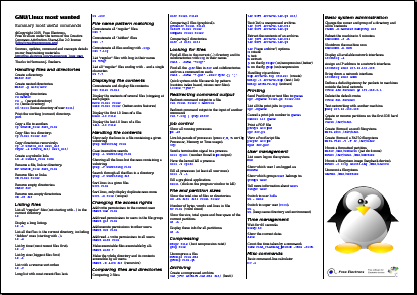
\includegraphics[width=\textwidth]{slides/course-information/command_memento.png}
  \end{columns}
\end{frame}

\begin{frame}
  \frametitle{vi basic commands}
  \begin{columns}
    \column{0.6\textwidth}
    \begin{itemize}
      \item The \code{vi} editor is very useful to make quick
      changes to files in a embedded target.
      \item Though not very user friendly at first, \code{vi}
      is very powerful and its main 15 commands are easy to
      learn and are sufficient for 99\% of everyone's needs!
      \item Get an electronic copy on
      \url{http://free-electrons.com/docs/command-line}
      \item You can also take the quick tutorial by running
      \code{vimtutor}. This is a worthy investment!
    \end{itemize}
    \column{0.4\textwidth}
    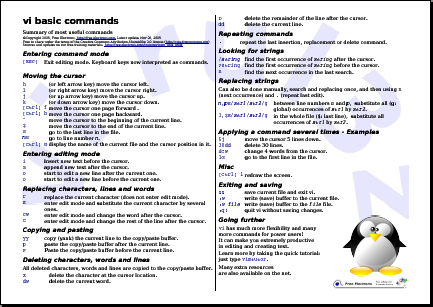
\includegraphics[width=\textwidth]{slides/header/vi_memento.png}
  \end{columns}
\end{frame}

